\part{Conception d'ensemble}
\setcounter{section}{0}

\section{Modèles conceptuels de données} 

\subsection{Données clients et produits} 

\begin{figure}[H]
\centering
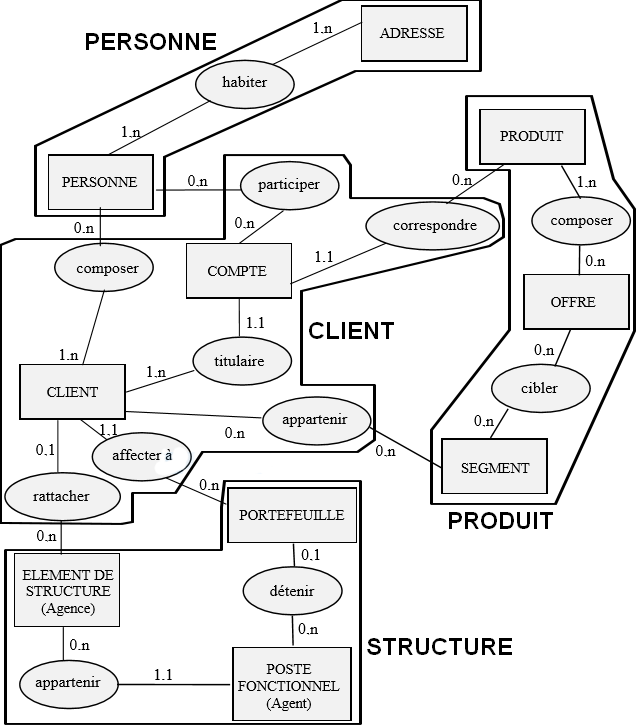
\includegraphics[width=\textwidth]{figures/mcd/MCD_Clients_Produits}
\caption{MCD Clients Produits}
\end{figure}


\subsection{Données commerciales}

\begin{figure}[H]
\centering
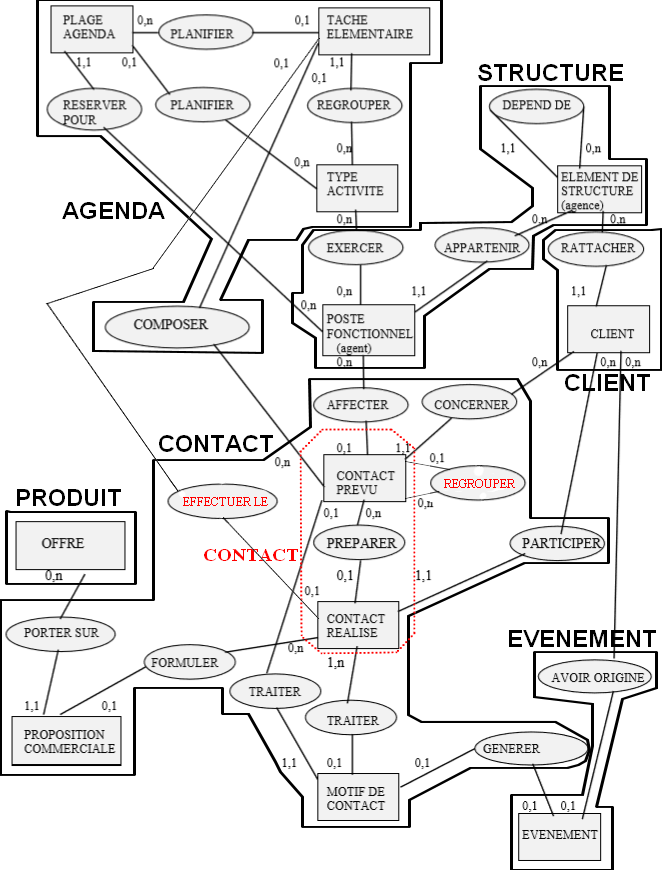
\includegraphics[width=\textwidth]{figures/mcd/MCD_Commercial}
\caption{MCD Commercial}
\end{figure}

\section{Diagramme d’état de l'objet métier \bf{contact}}

Le diagramme d'état suivant décrit le cycle de vie complet de l'objet \sc{Contact}. Le cas nominal concernant l'objet métier \sc{Contact} est le suivant, l'objet est créé automatiquement par le système suite à l'apparition d'un évènement entrainant sa création. Après cette action, l'objet contact est dans l'état \bf{PREVU}. Après affectation par le chef d'agence, l'objet \sc{Contact} atteint l'état \bf{AFFECTE} qui fait partie du super état \bf{EN TRAITEMENT}. L'agent est alors chargé de prendre rendez-vous avec le client ce qui a pour effet de faire passer le \sc{Contact} dans l'état \bf{RDV PRIS}. Depuis cet état l'agent peut préparer l'entretien et faire passer l'objet \sc{Contact} dans l'état \bf{PREPARE} puis conduire l'entretien et atteindre l'état \bf{REALISE} ou conduire l'entretien sans l'avoir préparé et atteindre directement \bf{REALISE}. Une fois dans cet état, l'objet \sc{Contact} n'évolue plus. \\
Quelques cas particuliers peuvent intervenir dans la vie de l'objet. Un \sc{Contact} peut être créé directement dans l'état \bf{RDV PRIS} sur contact spontané de la part du client. De même l'agent peut annuler le rendez-vous dans les états \bf{RDV PRIS} et \bf{PREPARE} faire passer l'objet \sc{Contact} dans l'état \bf{AFFECTE}. Enfin, l'agent peut annuler définitivement le contact depuis les états contenus dans le super état \bf{EN TRAITEMENT} ce qui a pour effet de faire passer l'objet \sc{Contact} dans l'état \bf{ANNULE} où il n'évolue plus.

\begin{figure}[H]
\noindent\makebox[\textwidth]{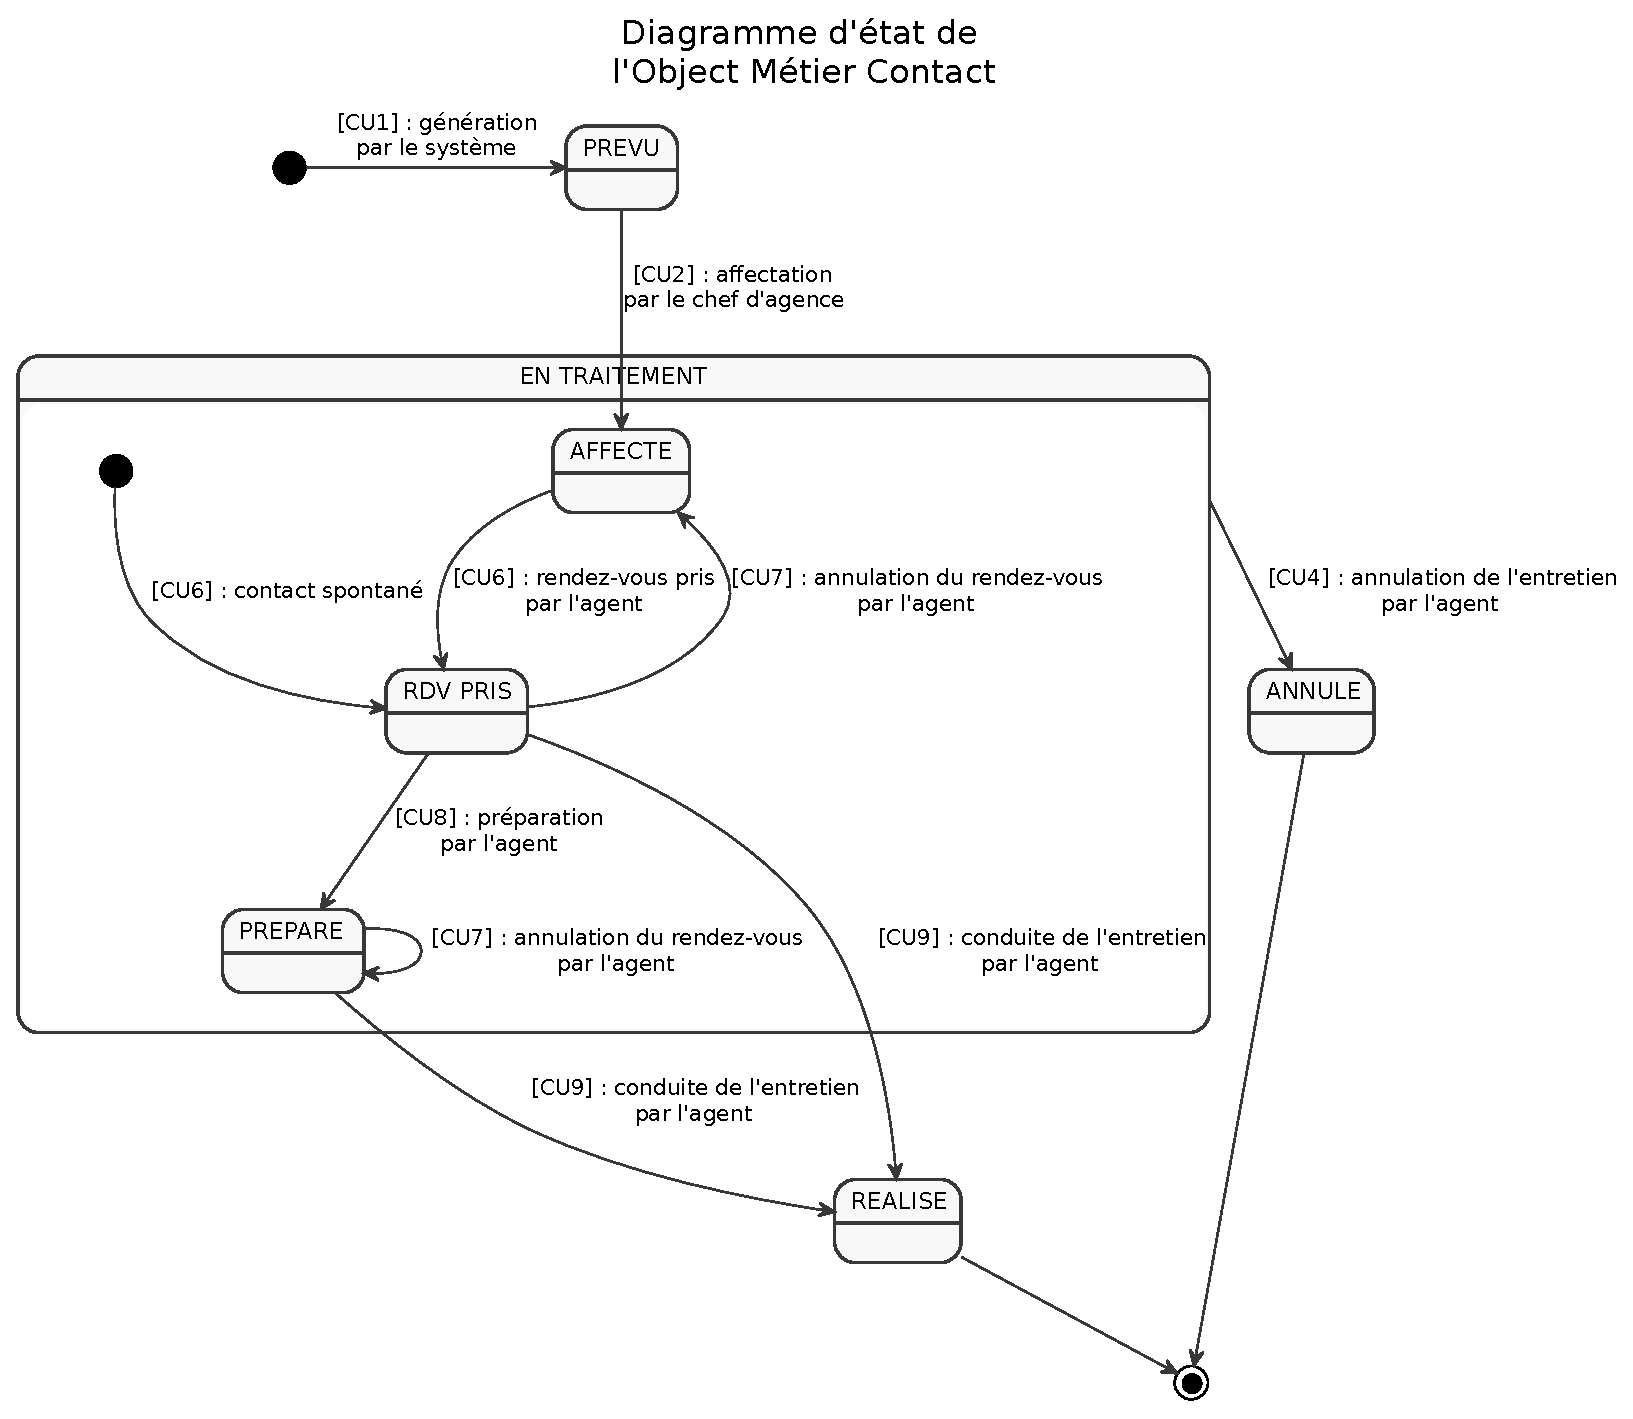
\includegraphics[width=18cm]{figures/eps/diag_etats_contact}}
\caption{Diagramme d'état de l'objet métier contact}
\end{figure}

\section{Choix  de  l’environnement  technique}
L’environnement  technique  déjà  retenu  par  la 
Maîtrise d’Ouvrage (MOA) de la banque est une architecture C/S n-tiers. 
